% \documentclass[12pt, twoside]{article}
\usepackage[letterpaper, margin=1in, headsep=0.2in]{geometry}
\setlength{\headheight}{0.6in}
%\usepackage[english]{babel}
\usepackage[utf8]{inputenc}
\usepackage{microtype}
\usepackage{amsmath}
\usepackage{amssymb}
%\usepackage{amsfonts}
\usepackage[nomessages]{fp} %\FPeval{\var-name}{2*sin(pi/6)}
\usepackage{siunitx} %units in math. eg 20\milli\meter
\usepackage{yhmath} % for arcs, overparenth command
\usepackage{tikz} %graphics
\usetikzlibrary{quotes, angles, arrows, arrows.meta}
\usepackage{graphicx} %consider setting \graphicspath{{images/}}
\usepackage{parskip} %no paragraph indent
\usepackage{enumitem}
\usepackage{multicol}
\usepackage{venndiagram}

\usepackage{fancyhdr}
\pagestyle{fancy}
\fancyhf{}
\renewcommand{\headrulewidth}{0pt} % disable the underline of the header
\raggedbottom
\hfuzz=2mm %suppresses overfull box warnings

\usepackage{hyperref}

\fancyhead[LE]{\thepage}
\fancyhead[RO]{\thepage \\ Name: \hspace{4cm} \,\\}
\fancyhead[LO]{BECA / Dr. Huson / Geometry\\*  Unit 9: Dilation \\* 18 January 2022}

\begin{document}

\subsubsection*{9.3 Homework: Overlapping triangles \hfill CCSS.HSG.SRT.B.5}
\begin{enumerate}
\item Each transformation we study--translation, dilation, rotation, and reflection--have specific details that must be stated to \emph{fully characterize} the transformation. Match the required details with the transformation.
  \begin{enumerate}[itemsep=0.5cm]
  \item The center, the degree measure and direction
  \item The line over which it is performed
  \item The horizontal and vertical distances
  \item The center and the scale factor $k$
  \end{enumerate}

\item A dilation centered at $A$ maps $\triangle ABC \rightarrow \triangle ADE$. Given that $BC = 10$, $DE = 15$.\\[0.5cm]
Write the value of the scale factor $k$ in the box.
    \begin{flushright}
      \begin{tikzpicture}[scale=0.8]
        \draw [-, thick] (0,0)--
        (6,0) node[below]{$E$}--
        (6,4.5) node[above right]{$D$}--cycle;
        \draw [thick] (4,0)--(4,3);
        \draw [fill] (0,0) circle [radius=0.1] node[below] {$A$};
        \node at (4,0) [below]{$C$};
        \node at (4,3) [above left]{$B$};
        %\node at (2, 0) [below]{$10$};
        %\node at (2, 2) [above]{$12$};
        \node at (6, 2.3) [right]{$15$};
        \node at (4, 1.5) [right]{$10$};
      \end{tikzpicture}
    \end{flushright}

\item A dilation centered at $A$ maps $\triangle ABC \rightarrow \triangle ADE$. Given that $BC = 8$, $DE = 14$.\\[0.5cm]
Write the value of the scale factor $k$ in the box.
    \begin{flushright}
      \begin{tikzpicture}[scale=0.8]
        \draw [-, thick] (0,0)--
        (6,0) node[below]{$E$}--
        (6,4.5) node[above right]{$D$}--cycle;
        \draw [thick] (4,0)--(4,3);
        \draw [fill] (0,0) circle [radius=0.1] node[below] {$A$};
        \node at (4,0) [below]{$C$};
        \node at (4,3) [above left]{$B$};
        %\node at (2, 0) [below]{$10$};
        %\node at (2, 2) [above]{$12$};
        \node at (6, 2.3) [right]{$14$};
        \node at (4, 1.5) [right]{$8$};
      \end{tikzpicture}
    \end{flushright}

\item A dilation centered at $A$ maps $\triangle ABC \rightarrow \triangle ADE$. Given that $BC = 9$, $DE = 15$.
\begin{enumerate}[itemsep=1.5cm]
  \item Find the value of the scale factor $k$.
  \item Given $AB=12$, find $AD$
  \item Given $AE=12.5$, find $AC$
\end{enumerate}
  \begin{flushright}
    \begin{tikzpicture}[scale=0.8]
      \draw [-, thick] (0,0)--
      (6,0) node[below]{$E$}--
      (6,4.5) node[above right]{$D$}--cycle;
      \draw [thick] (4,0)--(4,3);
      \draw [fill] (0,0) circle [radius=0.1] node[below] {$A$};
      \node at (4,0) [below]{$C$};
      \node at (4,3) [above left]{$B$};
      %\node at (2, 0) [below]{$10$};
      %\node at (2, 2) [above]{$12$};
      \node at (6, 2.3) [right]{$15$};
      \node at (4, 1.5) [right]{$9$};
    \end{tikzpicture}
  \end{flushright}

\item Dilate the triangle by a scale factor $k=2$ centered at the origin, $\triangle ABC \rightarrow \triangle A'B'C'$. Complete the table of the coordinates and plot and label the image on the grid. \vspace{0.5cm}
\begin{multicols}{2}
  $A(0,0) \rightarrow$ \\[0.7cm]
  $B(2,-2) \rightarrow$ \\[0.7cm]
  $C(2,0) \rightarrow$ \\[0.7cm]
    \begin{tikzpicture}[scale=.75]
    \draw [help lines] (-5,-5) grid (5,5);
    \draw [thick, <->] (-5.4,0) -- (5.4,0) node [right] {$x$};
    \draw [thick, <->] (0,-5.4)--(0,5.4) node [above] {$y$};  
    \draw [thick]
      (0,0) node[below left] {$A$}--
      (2,-2) node[below left] {$B$}--
      (2,0) node[above] {$C$}--cycle;  
    \end{tikzpicture}
  \end{multicols}

\item A dilation centered at $A$ maps $\triangle ABC \rightarrow \triangle ADE$. Given that $BC = 10$, $DE = 15$.
\begin{enumerate}[itemsep=1.5cm]
  \item Find the value of the scale factor $k$.
  \item Given $AB=12$, find $AD$
  \item Given $AE=12$, find $AC$
\end{enumerate}
  \begin{flushright}
    \begin{tikzpicture}[scale=1]
      \draw [-, thick] (0,0)--
      (5.25,0) node[below]{$E$}--
      (6,4.5) node[above right]{$D$}--cycle;
      \draw [thick] (3.5,0)--(4,3);
      \draw [fill] (0,0) circle [radius=0.1] node[below] {$A$};
      \node at (3.5,0) [below]{$C$};
      \node at (4,3) [above left]{$B$};
      %\node at (2, 0) [below]{$10$};
      %\node at (2, 2) [above]{$12$};
      \node at (5.8, 2.3) [right]{$15$};
      \node at (3.8, 1.5) [right]{$10$};
    \end{tikzpicture}
  \end{flushright}

\end{enumerate}
\end{document}
